\documentclass{article}

% Language setting
% Replace `english' with e.g. `spanish' to change the document language
\usepackage[english]{babel}

% Set page size and margins
% Replace `letterpaper' with `a4paper' for UK/EU standard size
\usepackage[letterpaper,top=2cm,bottom=2cm,left=3cm,right=3cm,marginparwidth=1.75cm]{geometry}

% Useful packages
\usepackage{amsmath}
\usepackage{graphicx}
\usepackage[colorlinks=true, allcolors=blue]{hyperref}
\title{Proyecto final}
\begin{document}
\maketitle
\section{Introduction}

Durante el desarrollo del siguiente proyecto en la primera parte desarrollamos ejercicios faciles de python en la cual observamos las diferencias en la sintaxis que existe a diferencia de c++ que es el lenguaje que se uso durante el curso.

En la segunda parte del proyecto todo los conceptos vistos en la primera parte en uno de los proyectos en la siguiente \href{https://www.freecodecamp.org/espanol/news/25-proyectos-en-python-para-principiantes/}{lista} en Python.

\section{Objetivos}

\subsection{Proporcionar a los estudiantes una introducción práctica al lenguaje Python, aplicando los conceptos aprendidos en C++ en un entorno diferente.
}
\subsection{Comprender las ventajas de Python en términos de sintaxis, productividad y aplicabilidad en diversas áreas tecnológicas tales como: inteligencia artificial, desarrollo web, ciencia de datos, etc.
}
\subsection{Ampliar sus habilidades de programación y perspectivas sobre el uso práctico de diferentes lenguajes de programación.
}

\section{Desarrollo (parte 1)}

A continuación, se presenta el desarrollo de seis códigos sencillos en Python, ideales para principiantes o para quienes deseen reforzar conceptos básicos de programación. Cada ejemplo incluye una breve explicación, el código y un análisis de su funcionamiento. 

\subsection*{1. Cálculo del Factorial de un Número}
El factorial de un número entero positivo $n$, denotado como $n!$, se define como el producto de todos los números enteros positivos desde 1 hasta $n$. Por ejemplo:
\[
5! = 5 \times 4 \times 3 \times 2 \times 1 = 120
\]
La función desarrollada utiliza una estructura condicional y un bucle para calcular el factorial.

\begin{center}
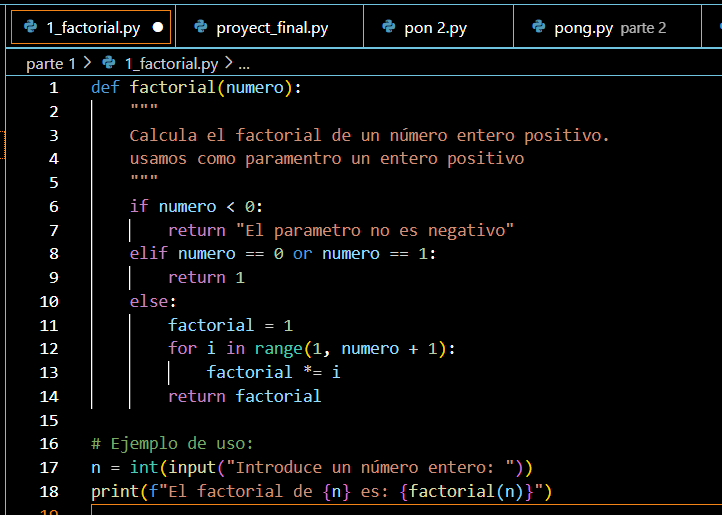
\includegraphics[width=\textwidth]{codigo1.jpg} % Inserta la imagen del código
\end{center}

\noindent \textbf{Resumen:} Este código verifica si el número ingresado es negativo, igual a 0 o 1, devolviendo el resultado correspondiente. Para otros casos, se utiliza un bucle para calcular el producto de los números desde 1 hasta el número ingresado.

\subsection*{2. Crear, Llenar e Imprimir una Matriz}
Este código permite al usuario crear una matriz, llenarla con valores ingresados desde el teclado e imprimirla en un formato legible. Es útil para aprender sobre listas anidadas y ciclos.

\begin{center}
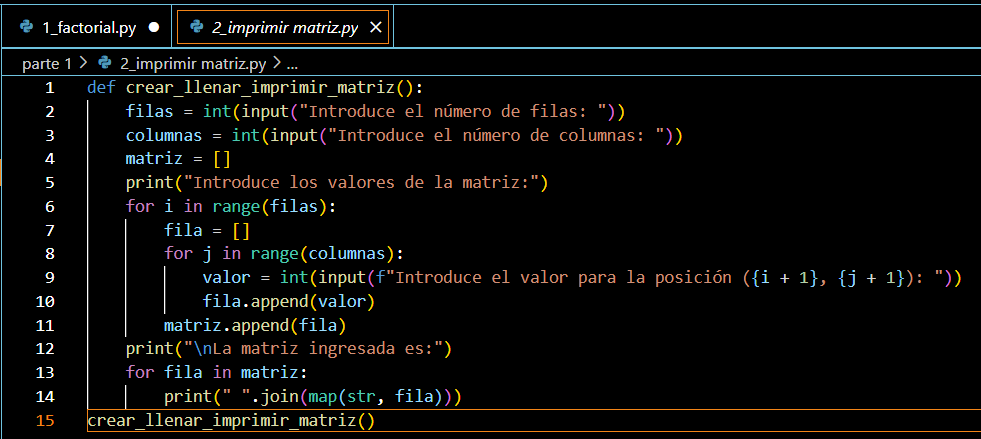
\includegraphics[width=\textwidth]{codigo2.jpg} % Inserta la imagen del código
\end{center}

\noindent \textbf{Resumen:} El usuario especifica el número de filas y columnas de la matriz. Luego, mediante ciclos anidados, se solicita el valor para cada posición, construyendo la matriz gradualmente. Finalmente, la matriz se imprime en un formato tabular.

\subsection*{3. Comprobación de una Cadena Palíndroma}
Un palíndromo es una palabra o frase que se lee igual hacia adelante y hacia atrás, ignorando espacios, puntuación y diferencias entre mayúsculas y minúsculas. Este código verifica si una cadena es palíndroma.

\begin{center}
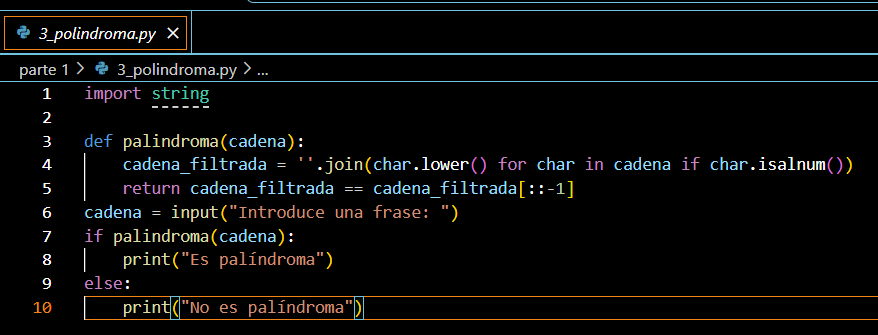
\includegraphics[width=\textwidth]{codigo3.jpg} % Inserta la imagen del código
\end{center}

\noindent \textbf{Resumen:} El código filtra caracteres no alfanuméricos y convierte la cadena a minúsculas. Luego, compara la cadena con su versión invertida para determinar si es palíndroma.

\subsection*{4. Gestión de Datos de un Estudiante}
Este código crea un diccionario para almacenar información sobre un estudiante, como su nombre, edad y promedio. Luego, se imprime la información de forma formateada.

\begin{center}
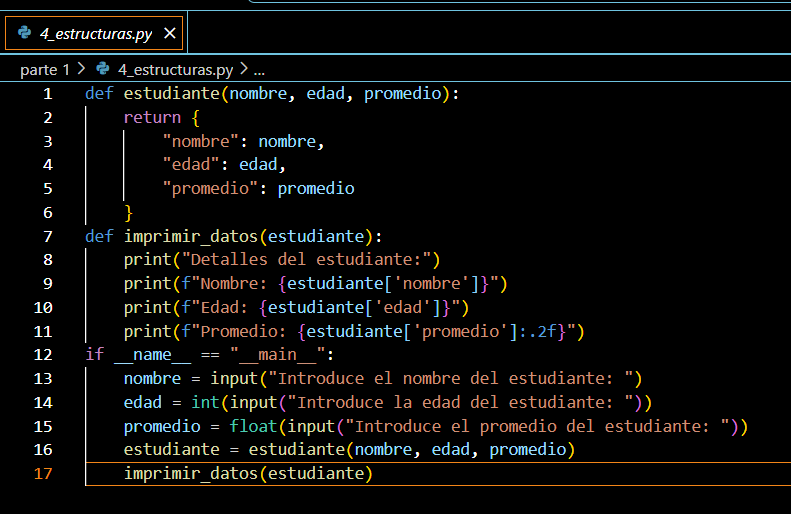
\includegraphics[width=\textwidth]{codigo4.jpg} % Inserta la imagen del código
\end{center}

\noindent \textbf{Resumen:} La función crea un diccionario que almacena los datos proporcionados por el usuario. Luego, otra función accede a este diccionario para presentar los datos del estudiante de manera estructurada.

\subsection*{5. Agregar Contenido a un Archivo}
Este programa permite agregar texto a un archivo existente. También incluye manejo de errores, como cuando el archivo no existe.

\begin{center}
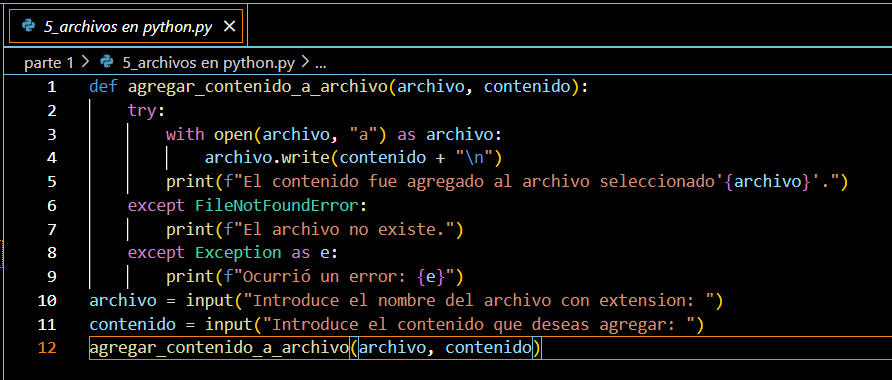
\includegraphics[width=\textwidth]{codigo5.jpg} % Inserta la imagen del código
\end{center}

\noindent \textbf{Resumen:} El programa abre el archivo en modo de adición (append) y agrega el contenido ingresado por el usuario. Si el archivo no existe, se maneja la excepción y se informa al usuario.

\subsection*{6. Simulación de Cuenta Bancaria}
Este programa utiliza una clase para simular operaciones básicas de una cuenta bancaria, como depositar, retirar y consultar el saldo.

\begin{center}
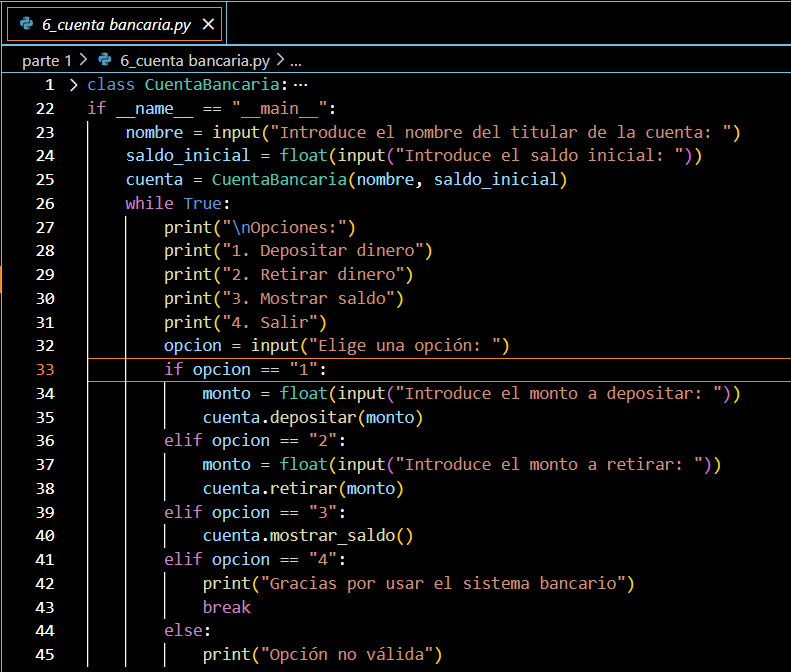
\includegraphics[width=\textwidth]{codigo6.jpg} % Inserta la imagen del código
\end{center}

\noindent \textbf{Resumen:} La clase \texttt{CuentaBancaria} define métodos para depositar, retirar y consultar el saldo de la cuenta. El programa incluye un menú interactivo para realizar las operaciones disponibles.

\section*{Parte 2}
Python es un lenguaje de programación ampliamente utilizado en diversos campos, incluido el desarrollo de videojuegos. Con bibliotecas como Pygame, permite a los desarrolladores crear experiencias interactivas y dinámicas de manera eficiente y accesible. En esta sección se explorará un proyecto práctico de desarrollo de un juego y los resultados obtenidos.

\subsection{Desarrollo de un juego en Python con Pygame}
En esta subsección se describe el desarrollo de un juego clásico tipo Pong utilizando Python y la biblioteca Pygame. El código implementa los siguientes elementos:

- **Superficie de dibujo y configuración inicial**: Se establece una ventana de 1000x600 píxeles con colores predeterminados para los objetos del juego.
- **Lógica de las palas**: Ambas palas son controladas por los jugadores, la izquierda con las teclas `W` y `S` y la derecha con las flechas `Arriba` y `Abajo`.
- **Movimiento y rebotes de la pelota**: La pelota se mueve continuamente y rebota al tocar las paredes o las palas.
- **Sistema de puntuación**: Se incrementa el puntaje cuando la pelota cruza los límites izquierdo o derecho.
- **Dibujado en pantalla**: Incluye la representación gráfica de las palas, la pelota, la línea central y el marcador.

El juego se ejecuta en un bucle principal controlado por el reloj de Pygame para mantener una tasa constante de fotogramas. El siguiente es un ejemplo visual del desarrollo:

\begin{figure}[h!]
    \centering
    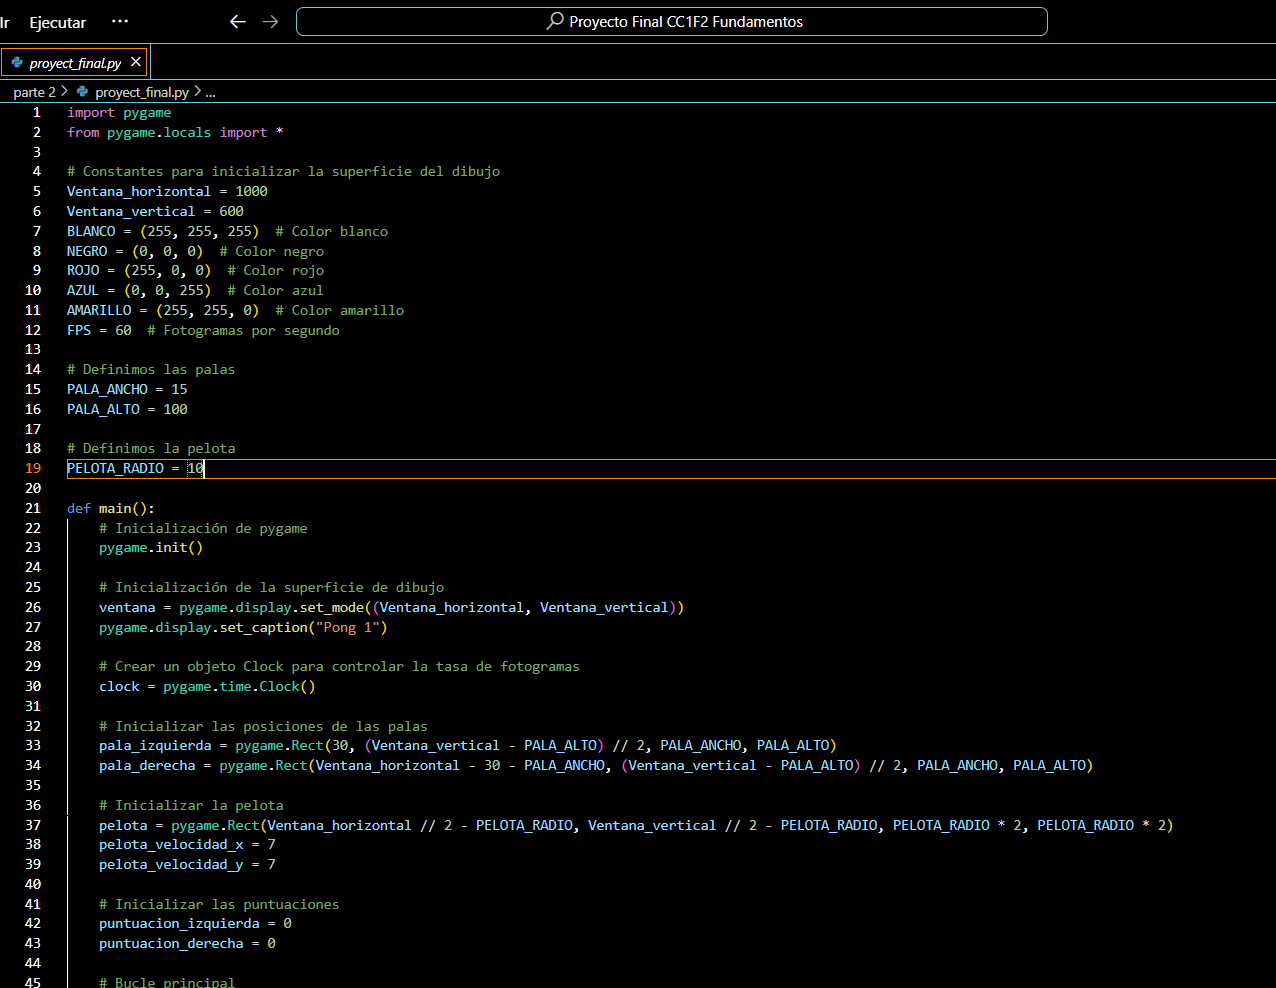
\includegraphics[width=0.7\textwidth]{pygame_desarrollo.png} % Cambia 'pygame_desarrollo.png' por el nombre de tu archivo
    \caption{Captura de pantalla del desarrollo del juego en Pygame.}
    \label{fig:pygame_desarrollo}
\end{figure}

\subsection{Explicación y resultados obtenidos}
En esta subsección se explica el proceso y los resultados obtenidos tras el desarrollo del juego. Se evaluará el diseño, la jugabilidad y el desempeño general del proyecto.

\begin{figure}[h!]
    \centering
    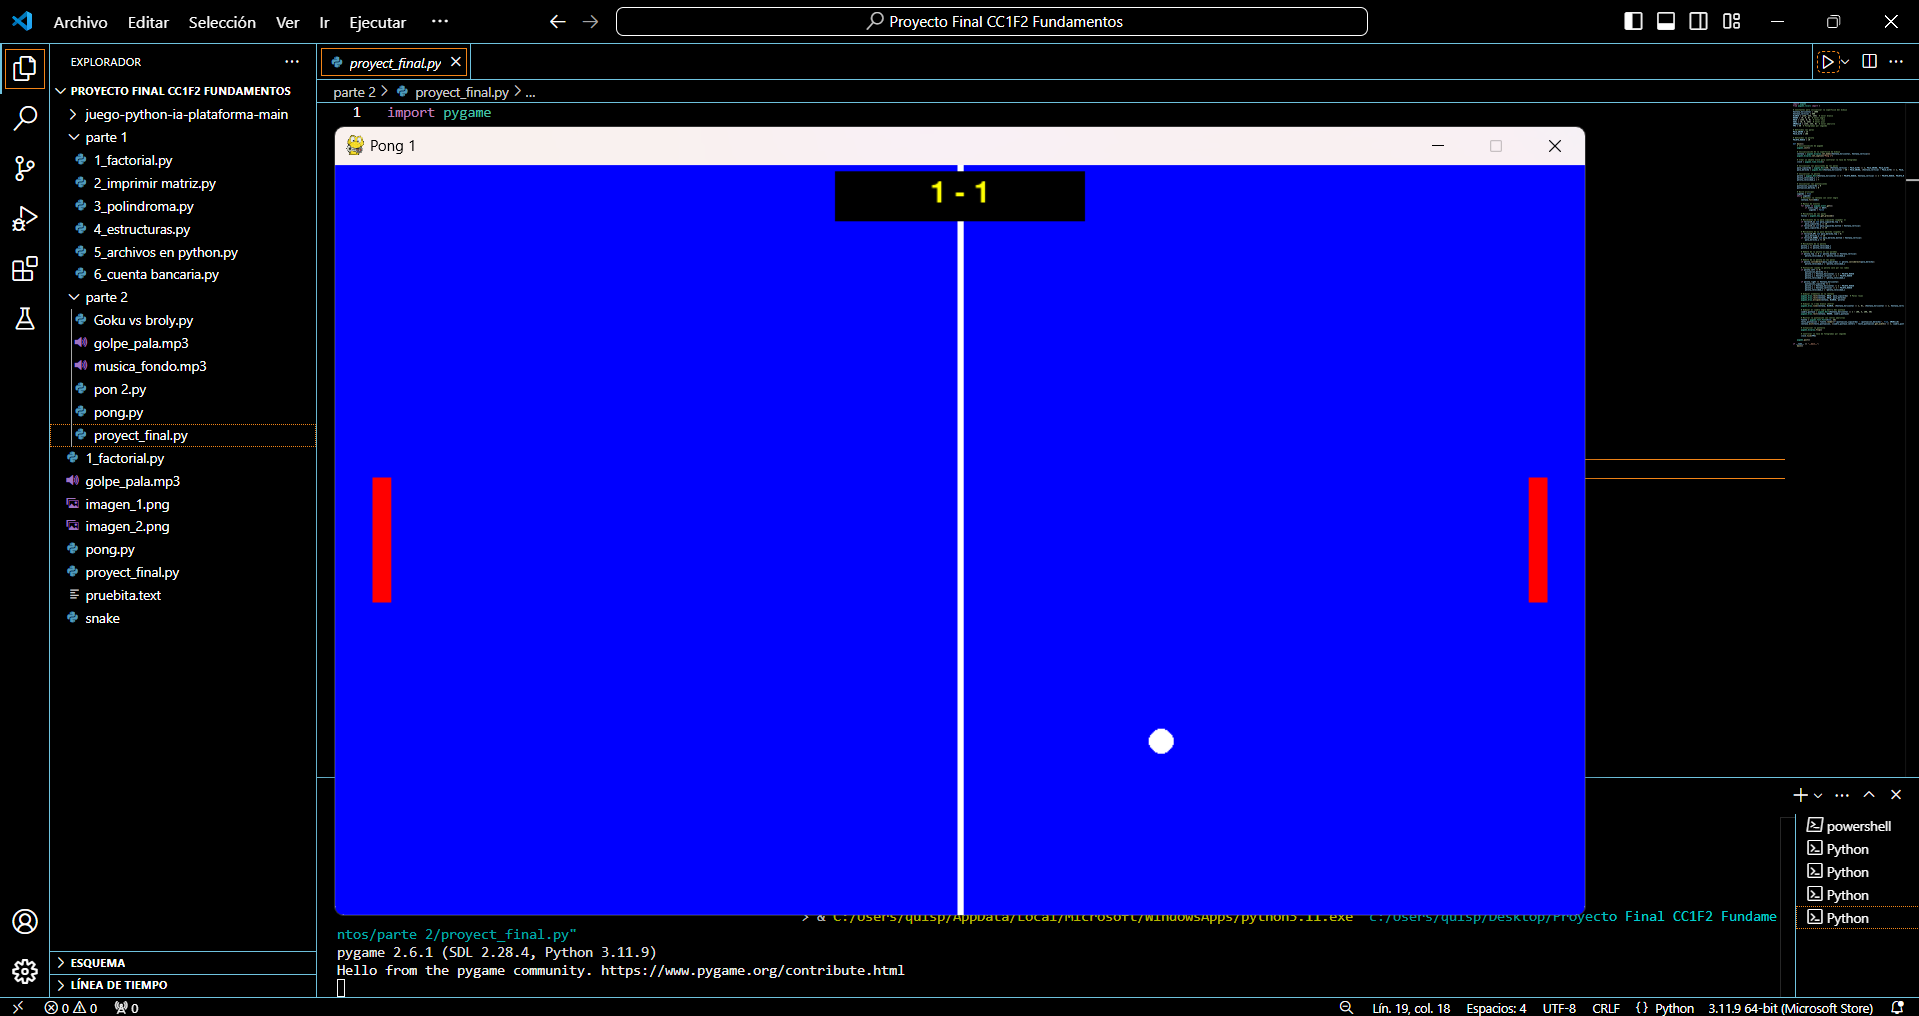
\includegraphics[width=0.7\textwidth]{resultados_obtenidos.png} % Cambia 'resultados_obtenidos.png' por el nombre de tu archivo
    \caption{Resultados obtenidos del juego desarrollado en Pygame.}
    \label{fig:resultados_obtenidos}
\end{figure}

\section*{Conclusiones}

El proyecto realizado, en el que se trabajaron los conceptos básicos de Python mediante seis códigos simples y la creación de un juego de Pong como parte final, ha sido de gran importancia tanto para el desarrollo de habilidades técnicas como para la comprensión práctica de la programación.

\subsection*{Conclusión}

El proyecto permitió al estudiante comprender de manera profunda y aplicada los conceptos fundamentales de Python, como variables, estructuras de control, funciones, y manipulación de datos. Los seis códigos simples sirvieron como ejercicios prácticos para familiarizarse con las herramientas básicas del lenguaje, mientras que el desarrollo del juego Pong representó un desafío que integró esos conceptos en una aplicación interactiva y visual.

\subsection*{Importancia del Proyecto}

\begin{itemize}
    \item \textbf{Refuerzo de los conceptos básicos}: A través de los seis códigos simples, el estudiante tuvo la oportunidad de experimentar con lo aprendido, resolver problemas y corregir errores, lo cual refuerza el conocimiento teórico de Python.
    
    \item \textbf{Desarrollo de habilidades prácticas}: El proyecto del juego Pong permitió aplicar esos conceptos en un contexto más complejo, fomentando el pensamiento lógico y la resolución de problemas. Crear un juego de esta índole no solo mostró cómo escribir código funcional, sino cómo integrar distintos elementos (como gráficos, interacción y lógica) en una sola aplicación.
    
    \item \textbf{Preparación para futuros proyectos}: El desarrollo de un juego no solo fue un ejercicio de programación, sino una experiencia que prepara al estudiante para proyectos más avanzados. Aprender a trabajar con librerías, como las que se utilizan para gráficos o interacción en Python, y desarrollar una aplicación completa, representa una habilidad esencial para proyectos más complejos en el futuro.
    
    \item \textbf{Motivación y creatividad}: Al concluir un proyecto tangible como un juego, el estudiante se siente motivado al ver los resultados de su trabajo. Además, el proyecto ofreció una plataforma para explorar la creatividad, al decidir cómo estructurar el juego y qué características incluir, lo que puede inspirar el desarrollo de futuros proyectos innovadores.
\end{itemize}

En resumen, este proyecto no solo consolidó el conocimiento básico de Python, sino que también mostró la relevancia de esos conceptos en la creación de aplicaciones funcionales, siendo un paso crucial en el camino hacia el dominio completo del lenguaje y la programación en general.

\section*{Referencias}

\begin{itemize}
    \item FreeCodeCamp: \url{https://www.freecodecamp.org/}
    \item Python Oficial: \url{https://www.python.org/}
\end{itemize}

\end{document}
